\documentclass[tikz,border=2pt]{standalone}
\renewcommand{\familydefault}{\sfdefault}
\usetikzlibrary{arrows.meta,calc,positioning}
\tikzset{every picture/.style={line width=1pt, >=Stealth},
         hl/.style={fill=black, fill opacity=0.12, text opacity=1}}
\usetikzlibrary{shapes.geometric}
\begin{document}
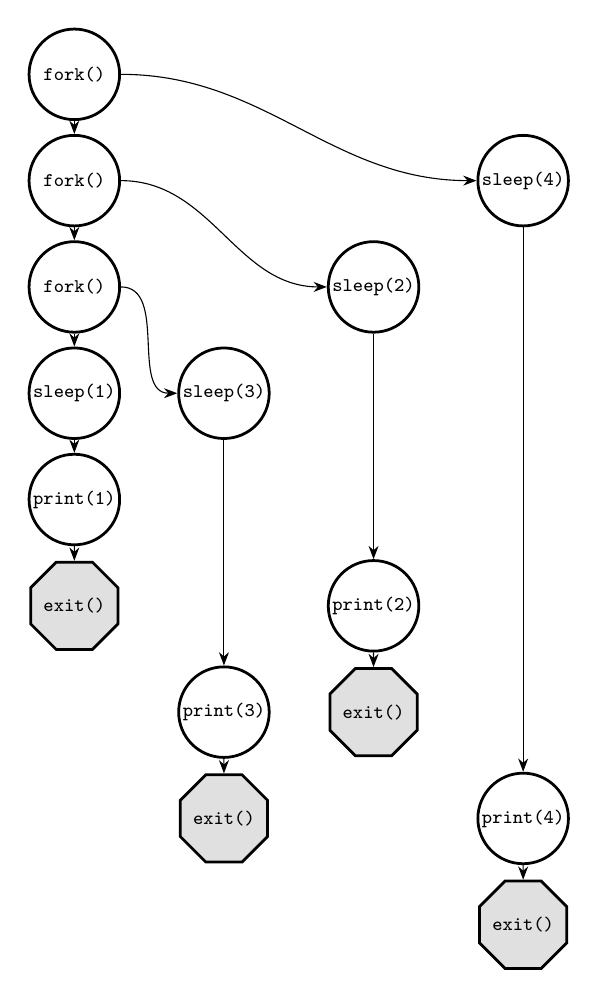
\begin{tikzpicture}[x=1.9cm, y=-1.35cm, op/.style={draw, circle, minimum size=1.15cm, inner sep=0pt, font=\ttfamily\scriptsize},
    end/.style={op, regular polygon, regular polygon sides=8, hl}]
  % The parent (left column) forks three times; child k sleeps k seconds, prints k, and exits.
  % Rows run down in time order, so the prints appear in the order 1, 2, 3, 4.
  \foreach \k/\y in {1/0, 2/1, 3/2} \node[op] (fork\k) at (0, \y) {fork()};
  \node[op] (s1) at (0, 3) {sleep(1)};
  \node[op] (p1) at (0, 4) {print(1)};
  \node[end] (e1) at (0, 5) {exit()};
  \foreach \a/\b in {fork1/fork2, fork2/fork3, fork3/s1, s1/p1, p1/e1} \draw[->, thin] (\a) -- (\b);
  \foreach \k/\x/\start in {4/3/1, 2/2/2, 3/1/3} {
    \node[op] (s\k) at (\x, \start) {sleep(\k)};
    \node[op] (p\k) at (\x, \k + 3) {print(\k)};
    \node[end] (e\k) at (\x, \k + 4) {exit()};
    \draw[->, thin] (s\k) -- (p\k);
    \draw[->, thin] (p\k) -- (e\k);
  }
  \draw[->, thin] (fork1) to[out=0, in=180] (s4);
  \draw[->, thin] (fork2) to[out=0, in=180] (s2);
  \draw[->, thin] (fork3) to[out=0, in=180] (s3);
\end{tikzpicture}
\end{document}
